% !TEX root = thesis.tex
\chapter{Background}
\label{chap:background}
In this chapter we describe the background techniques and tools used in our research. Specifically we cover mutation testing in Section~\ref{sec:background_mutation_testing}, machine learning in Section~\ref{sec:background_machine_learning} and software metrics in Section~\ref{sec:background_metrics}.


\section{Mutation Testing}
\label{sec:background_mutation_testing}
As mentioned in Section~\ref{sec:introduction_motivation} there exists techniques that measure code coverage. Mutation testing can be seen as a fault-based coverage technique that demonstrate the absence of faults in a software system~\cite{DLS78, BSLS80}. Mutation testing makes use of fault-based testing by generating a set of mutants, each representing a possible fault in the software system. These mutants are then executed along with the test suite with hopes that the test suite can detect the mutant's fault. If the fault is detected this means that the test suite is effective enough to handle the detection of that specific bug. If the fault goes undetected then the test suite is lacking as it cannot detect that specific bug. Using the results of mutation testing it is possible to assess the adequacy of a test suite -- the effectiveness of the test suite of detecting bugs.

\begin{figure}[t!]
  \centering
  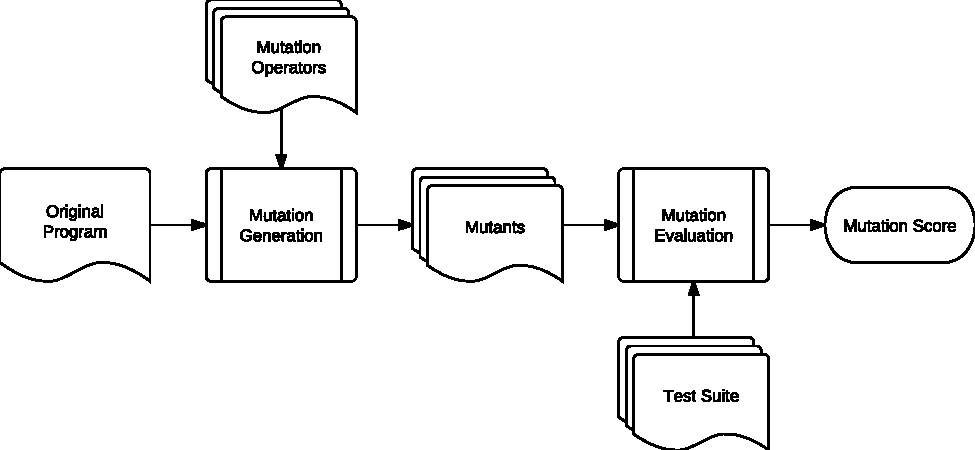
\includegraphics[width=14cm]{figures/mutation_testing_overview.pdf}
  \caption{The mutation testing process.}
  \label{fig:mutation_testing_overview}
  \vspace{2mm}
  \hrule
\end{figure}

Figure~\ref{fig:mutation_testing_overview} illustrates a general approach to mutation testing. Mutation testing uses a set of \emph{mutation operators} to generate faulty versions of a software system's source code called \emph{mutants}. A mutation operator applies a transformation to a software artifact such that it now exhibits a fault (see Section~\ref{subsubsec:background_method_operators} for examples). Mutation operators are designed based on existing fault taxonomy, such that the generate mutants that represent real faults. Studies have indicated that mutants could be used as substitutes for real faults~\cite{ABLN06, ABL05, NK11}.

The transformation of a software artifact to create a mutant is typically a small/single change as most bugs appear follow the \emph{\gls{cph}}~\cite{ABD+79} which suggests that developers write software that is nearly correct. The \emph{\gls{ceh}}~\cite{Off92} suggests that a large percent of complex faults can be detected if all the simple faults can be detected. These two hypothesis strengthen the use of simple small changes for mutation operators and why mutation testing is adequate for evaluating test suite effectiveness.

\begin{equation}
  \emph{$\text{mutation score} = \frac{\text{killed mutants}}{\text{total mutants} - \text{equivalent mutants}}$}
  \label{equ:mutation_score}
\end{equation}

After all the mutants have been generated a testing approach is used to evaluate them against the test suite. If a mutant is detected by the test suite then the mutant is \emph{killed} otherwise it has \emph{survived}. There are some cases where the mutant generated is \emph{equivalent} such that the behaviour of the mutant is the same as the original system. These equivalent mutants pose a problem as they cannot be killed using the given test suite. Manual inspection of mutants to determine if they are equivalent is not feasible for a large number of mutants. A \emph{mutation score} is given to each source code unit based on the number of percentage of non-equivalent mutants they killed. The mutation score indicates how effective a test suite is at detecting faults in terms of mutation fault-based testing adequacy.

Mutation testing has traditionally been used as a coverage technique to evaluate the effectiveness of test suites and provide confidence in the testing process~\cite{JH10}. For over 30 years, mutation testing has been applied to software written in programming languages including C~\cite{DM96, JH08}, Fortran~\cite{KO91} and Java~\cite{MKO02, BCD06}. Furthermore, mutation testing has also been applied to non-programming artifacts such as formal specification languages~\cite{ABM98}, markup languages~\cite{PO10} and spreadsheets~\cite{AE09}.

The following present the two major criticisms of mutation testing, accompanied with some of the research has been done to alleviate these to some degree:

\begin{itemize}
	\item \textbf{Equivalent Mutants:} As already described these are mutants that semantically the same as the original version of the software system. An equivalent mutant will not be killed by the test suite and this results in lower than expected mutation scores. These are problematic as mutation score is influenced by these mutants though they are difficult/costly to detect. Schuler et al. proposes a solution in determining whether a surviving mutant is equivalent or not using impact analysis~\cite{SZ10}. Their approach observes the impact of the original program's execution against that of the mutant in respect to control flow and data. Their experiments showed that using statement coverage allowed them to achieved a classification precision of 75\% and a recall of 56\%. In their previous work they also considered the use of the impact of dynamic invariants to uncover equivalent mutants~\cite{SDZ09}. Offutt et al. used compiler optimization techniques and were able to detect about 10\% of equivalent mutations~\cite{OC94}.
	\item \textbf{Performance Cost:} Again as we have already mentioned mutation testing is a very costly coverage technique as many mutants must be evaluated against the test suite. The mutant representation, selection of tests, strategies are all aspects of the mutation testing process that the research community are exploring to reduce cost. Mutation sampling can be used to reduce the evaluation efforts by only considering a random subset of the generated mutants~\cite{Bud80}. Untch et al. introduced a mutation runtime technique call \emph{Mutant Schema Generation} that represented all possible mutants in a single meta-program~\cite{UOH93}. Offutt et al. were able to perform mutation testing at the bytecode level, effectively avoiding recompilations of the generated mutants~\cite{OMK04}.
\end{itemize}

\subsection{Mutation Operators}
\label{subsec:background_mutation_operators}
As previous mentioned mutation operators define transformations that attempts to introduce faults. Focusing on Java there two common sets of mutation operators: method-level and class-level. We list and describe these two sets of mutation operators in the following sections.


\subsubsection{Method-Level Mutation Operators}
\label{subsubsec:background_method_operators}
\begin{table}[t!]
  \centering
  \rowcolors{2}{gray!30}{gray!20}
  \begin{tabular}{|l|l|}
    \hline
    \rowcolor[RGB]{169,196,223}
    \textbf{Operator} & \textbf{Description} \\
    \hline AOR & Arithmetic Operator Replacement \\
    \hline AOI & Arithmetic Operator Insertion \\
    \hline AOD & Arithmetic Operator Deletion \\
    \hline ROR & Relational Operator Replacement \\
    \hline COR & Conditional Operator Replacement \\
    \hline COI & Conditional Operator Insertion \\
    \hline COD & Conditional Operator Deletion \\
    \hline SOR & Shift Operator Replacement \\
    \hline LOR & Logical Operator Replacement \\
    \hline LOI & Logical Operator Insertion \\
    \hline LOD & Logical Operator Deletion \\
    \hline ASR & Assignment Operator Replacement \\
    \hline
  \end{tabular}
  \caption{The set of method-level mutation operators from the MuJava mutation testing tool~\cite{MOK05, MO05a}.}
  \label{tab:method_operators}
  \vspace{2mm}
  \hrule
\end{table}

We first consider the set of method-level mutation operators found in the mutation testing tool \emph{MuJava}~\cite{MOK05}, as they are well documented and designed. These mutation operators apply source transformations that modify expressions at the method-level. These operators can cause unexpected data values to occur, as well as adjusting the outcome of conditions. Figure~\ref{tab:method_operators} lists a set of method-level mutation operators~\cite{MO05a}.

\begin{figure}[t!]
  \centering
  \begin{minipage}{6.5cm}
  \centering
  \footnotesize{\textbf{Original Program}}
  \lstinputlisting[language=Java, literate={>}{{\textcolor{red}{>}}}{1}]{listings/mutation_example.java}
  \end{minipage}
  $\xrightarrow{\texttt{ROR}}$
  \begin{minipage}{6.5cm}
  \centering
  \footnotesize{\textbf{Mutant Program}}
  \lstinputlisting[language=Java, literate={>}{{\textcolor{red}{<}}}{1}]{listings/mutation_example.java}
  \end{minipage}
  \caption{Example application of the \texttt{ROR} method-level mutation operator.}
  \vspace{2mm}
  \hrule
  \label{fig:ROR_mutation}
\end{figure}

\begin{figure}[t!]
  \centering
  \begin{minipage}{6.5cm}
  \centering
  \footnotesize{\textbf{Original Program}}
  \lstinputlisting[language=Java, literate={this.limit}{{\textcolor{red}{\textbf{this}.limit}}}{10}]{listings/mutation_example.java}
  \end{minipage}
  $\xrightarrow{\texttt{AOI}}$
  \begin{minipage}{6.5cm}
  \centering
  \footnotesize{\textbf{Mutant Program}}
  \lstinputlisting[language=Java, literate={this.limit}{{\textcolor{red}{\textbf{this}.limit---}}}{12}]{listings/mutation_example.java}
  \end{minipage}
  \caption{Example application of the \texttt{AOI} method-level mutation operator.}
  \vspace{2mm}
  \hrule
  \label{fig:AOI_mutation}
\end{figure}

To illustrate the effects of a method-level operator, consider the \emph{Relational Operator Relational} (\texttt{ROR}) mutation operator. This mutation operator replaces a relational operator (i.e., \texttt{>}, \texttt{>=}, \texttt{==}, \texttt{!=}, \texttt{=<} or, \texttt{<}) with another type of relational operator as seen in Figure~\ref{fig:ROR_mutation}. Figure~\ref{fig:AOI_mutation} presents another example demonstrating the \emph{Arithmetic Operator Insertion} (\texttt{AOI}) mutation operator. The remaining set of method-level mutation operators function in a similar fashion except with other operators (i.e., conditional, shift, logical and, assignment).

\subsubsection{Class-Level Mutation Operators}
\label{subsubsec:background_class_operators}
\begin{table}[t!]
  \centering
  \rowcolors{2}{gray!30}{gray!20}
  \begin{tabular}{|c|l|l|}
    \hline
    \rowcolor[RGB]{169,196,223}
    \textbf{Group} & \textbf{Operator} & \textbf{Description} \\
    \hline \ding{172} & AMC & Access modifier change \\
    \hline \ding{173} & IHD & Hiding variable deletion \\
    \hline \ding{173} & IHI & Hiding variable insertion \\
    \hline \ding{173} & IOD & Overriding method deletion \\
    \hline \ding{173} & IOP & Overriding method calling position change \\
    \hline \ding{173} & IOR & Overriding method rename \\
    \hline \ding{173} & ISI & \texttt{super} keyword insertion \\
    \hline \ding{173} & ISD & \texttt{super} keyword deletion \\
    \hline \ding{173} & IPC & Explicit call to a parent's constructor deletion \\
    \hline \ding{174} & PNC & \texttt{new} method call with child class type \\
    \hline \ding{174} & PMD & Member variable declaration with parent class type \\
    \hline \ding{174} & PPD & Parameter variable declaration with child class type \\
    \hline \ding{174} & PCI & Type cast operator insertion \\
    \hline \ding{174} & PCC & Cast type change \\
    \hline \ding{174} & PCD & Type cast operator deletion \\
    \hline \ding{174} & PRV & Reference assignment with other comparable variable \\
    \hline \ding{174} & OMR & Overloading method contents replace \\
    \hline \ding{174} & OMD & Overloading method deletion \\
    \hline \ding{174} & OAC & Arguments of overloading method call change \\
    \hline \ding{175} & JTI & \texttt{this} keyword insertion \\
    \hline \ding{175} & JTD & \texttt{this} keyword deletion \\
    \hline \ding{175} & JSI & \texttt{static} modifier insertion \\
    \hline \ding{175} & JSD & \texttt{static} modifier deletion \\
    \hline \ding{175} & JID & Member variable initialization deletion \\
    \hline \ding{175} & JDC & Java-supported default constructor creation \\
    \hline \ding{175} & EOA & Reference assignment and content assignment replacement \\
    \hline \ding{175} & EOC & Reference comparison and content comparison replacement \\
    \hline \ding{175} & EAM & Acessor method change \\
    \hline \ding{175} & EMM & Modifier method change \\
    \hline
  \end{tabular}
  \caption{The set of class-level mutation operators from the MuJava mutation testing tool~\cite{MOK05, MO05b}.}
  \vspace{1mm}
  \footnotesize{\emph{The group column indicates the specific language feature of the mutation operator (\ding{172}: Encapsulation, \ding{173}: Inheritance, \ding{174}: Polymorphism, \ding{175}: Java-Specific Features).}}
  \vspace{2mm}
  \hrule
  \label{tab:class_operators}
\end{table}

We now look at the set of class-level mutation operators found in \emph{MuJava}~\cite{MOK05, MKO02}. These mutation operators apply source transformations that modify language features at the class-level. These operators can allow objects to behave in unexpected ways, as well as exposing design issues. Figure~\ref{tab:class_operators} tabulates the class-level mutation operators~\cite{MO05b}.

\begin{figure}[b!]
  \centering
  \begin{minipage}{6.5cm}
  \centering
  \footnotesize{\textbf{Original Program}}
  \lstinputlisting[language=Java, literate={Integer\ limit\ =\ new\ Integer(10)}{{{\textcolor{red}{Integer\ limit\ =\ \textbf{new}\ Integer(10)}}}}{31}]{listings/mutation_example.java}
  \end{minipage}
  $\xrightarrow{\texttt{JID}}$
  \begin{minipage}{6.5cm}
  \centering
  \footnotesize{\textbf{Mutant Program}}
  \lstinputlisting[language=Java, literate={Integer\ limit\ =\ new\ Integer(10)}{{{\textcolor{red}{Integer\ limit}}}}{13}]{listings/mutation_example.java}
  \end{minipage}
  \caption{Example application of the \texttt{JID} class-level mutation operator.}
  \vspace{2mm}
  \hrule
  \label{fig:JID_mutation}
\end{figure}

\begin{figure}[t!]
  \centering
  \begin{minipage}{6.5cm}
  \centering
  \footnotesize{\textbf{Original Program}}
  \lstinputlisting[language=Java, literate={public}{{\textbf{\textcolor{red}{public}}}}{6}]{listings/mutation_example.java}
  \end{minipage}
  $\xrightarrow{\texttt{AMC}}$
  \begin{minipage}{6.5cm}
  \centering
  \footnotesize{\textbf{Mutant Program}}
  \lstinputlisting[language=Java, literate={public}{{\textbf{\textcolor{red}{private}}}}{7}]{listings/mutation_example.java}
  \end{minipage}
  \caption{Example application of the \texttt{AMC} class-level mutation operator.}
  \vspace{2mm}
  \hrule
  \label{fig:AMC_mutation}
\end{figure}

To illustrate the effects of a class-level operator, we can look at the \emph{Member Variable Initialization Deletion} (\texttt{JID}) mutation operator. This mutation operator deletes an instance variables initialization as sees in Figure~\ref{fig:JID_mutation}. Figure~\ref{fig:AMC_mutation} presents another example demonstrating the \emph{Access Modifier Change} (\texttt{AMC}) mutation operator. The remaining set of class-level mutation operators function by inserting, deleting and, changing certain elements in the class with respect to inheritance, polymorphism, and Java-specific features.


\subsubsection{Other Mutation Operators}
\label{subsubsec:background_other_operators}
In addition to the two general sets of mutation operators just described, sets also exist for specify domains (i.e., concurrency and security). Bradbury et. al. presented a set of concurrency mutation operators that is capable of creating data races and deadlock faults~\cite{BCD06}. Shahrair et al. presented multiple sets of mutation operators in the security domain for database injection~\cite{SZ08b}, buffer overflows\cite{SZ08} and cross site scripting~\cite{SZ08a}. Furthermore, as mentioned earlier on in Section~\ref{sec:background_mutation_testing} other domains where mutation testing has been applied have their own set of mutation operators (i.e., spreadsheets, markup), though this is outside the scope of this thesis.


\subsection{Mutation Testing Tools}
\label{subsec:background_mutation_tools}
In the last decade a number of mutation testing tools for the Java programming language have emerged~\cite{JH10}. We present the following set of criteria that distinguishes most of the tools from each other:

\begin{itemize}
  \item \textbf{Inception Year}: the year the tool was released to the public.
  \item \textbf{Generation-Level}: mutation can be generated either at the source code or bytecode level. Source code mutation generation requires re-compilation, while bytecode does not.
  \item \textbf{Test Selection}: test selection indicates which unit test cases are ran for each mutant. A naive based approach simply runs all the unit test cases, while convention based runs all tests based on a package/test name or defined annotations. Coverage based approach only runs unit test cases that are directly involved in the mutated source code, while a manual bases approach allows the user to specify each unit test case.
  \item \textbf{Mutant Insertion}: generated mutants are stored and ran against the selected unit test cases. A naive approach stores the mutants on disk and creates a new \gls{jvm} for each mutant. A schmeta~\cite{UOH93} approach stores all the mutants in a single class, and the mutants are enabled through runtime flags one-at-a-time. An in-memory approach stores all the mutants in-memory which are then injected into the \gls{jvm} by creating a new classloader. An instrumentation approach stores the mutants in memory, but injects them into the \gls{jvm} directly using an instrumentation \gls{api}.
  \item \textbf{Method-Level}: whether a tool has a set of \emph{traditional} method-level mutation operators as mentioned in Section~\ref{subsubsec:background_method_operators}.
  \item \textbf{Class-Level}: whether a tool has a set of object-oriented class-level mutation operators as mentioned in Section~\ref{subsubsec:background_class_operators}.
  \item \textbf{Concurrency-Level}: whether a tool has a set of concurrency-level mutation operators, those which mutate concurrency syntax to cause potential deadlocks, data races and more concurrency related bugs.
  \item \textbf{JUnit Support}: whether a tool has support for JUnit test cases (de facto for unit testing Java~\cite{JUnit}.
  \item \textbf{Command-Line}: whether a tool has support to be ran via a command-line interface.
  \item \textbf{Structured Output}: whether a tool has support to output results in a structure format (i.e., \gls{xml}, \gls{csv})
  \item \textbf{Unit Scores}: whether a tool indicates the mutation score of individual source code units (i.e., the mutation score of methods).
  \item \textbf{Open Source}: whether a tool's source code is open source and freely available to modify.
  \item \textbf{Academic Tool}: whether a tool was developed from an academic research group, otherwise industry or community developed.
  \item \textbf{Special Feature}: whether a tools has a special feature that is unique in mutation testing.
\end{itemize}

\begin{landscape}
  \begin{table}[t!]
    \centering
    \rowcolors{1}{gray!30}{gray!20}
    \begin{threeparttable}
      \begin{tabular}{|l|l|l|l|l|l|l|}
        \rowcolor[RGB]{169,196,223}
        \hline & \textbf{Jester~\cite{Jester}} & \textbf{MuJava~\cite{MOK05}} & \textbf{Jumble~\cite{Jumble}} & \textbf{Javalanche~\cite{SZ09}} & \textbf{Judy~\cite{MR10}} & \textbf{PIT~\cite{PIT}} \\
        \hline \cellcolor[RGB]{169,196,223} \textbf{Inception Year} & 2001 & 2004 & 2007 & 2009 & 2010 & 2011 \\
        \hline \cellcolor[RGB]{169,196,223} \textbf{Generation-Level} & Source Code & Bytecode & Bytecode & Bytecode & Source Code & Bytecode \\
        \hline \cellcolor[RGB]{169,196,223} \textbf{Test Selection} & Naive\tnote{f} & Manual & Convention & Coverage & Convention & Coverage \\
        \hline \cellcolor[RGB]{169,196,223} \textbf{Mutant Insertion} & Naive\tnote{f} & Schmeta & In-Memory & Schmeta & Schmeta\tnote{c} & Instrument \\
        \hline \cellcolor[RGB]{169,196,223} \textbf{Method-Level} & No & Yes & No & Yes & Yes & Yes \\
        \hline \cellcolor[RGB]{169,196,223} \textbf{Class-Level} & No & Yes & No & No & Yes\tnote{b} & No \\
        \hline \cellcolor[RGB]{169,196,223} \textbf{Concurrency-Level} & No & No & No & Yes & No & No \\
        \hline \cellcolor[RGB]{169,196,223} \textbf{JUnit Support} & Yes & No\tnote{c} & Yes & Yes & Yes & Yes \\
        \hline \cellcolor[RGB]{169,196,223} \textbf{Command-Line} & Yes & No & Yes & Yes & Yes & Yes \\
        \hline \cellcolor[RGB]{169,196,223} \textbf{Structured Output} & No & No & No & Yes & No & Yes \\
        \hline \cellcolor[RGB]{169,196,223} \textbf{Unit Scores} & No & No & No & Yes & No & No\tnote{g} \\
        \hline \cellcolor[RGB]{169,196,223} \textbf{Open Source} & Yes & No\tnote{d} & Yes & Yes & No & Yes \\
        \hline \cellcolor[RGB]{169,196,223} \textbf{Academic Tool} & No & Yes & No & Yes & Yes & No \\
        \hline \cellcolor[RGB]{169,196,223} \textbf{Special Feature} & No & No & No & Yes\tnote{e} & No & No \\
        \hline
      \end{tabular}
      \begin{tablenotes}
        \item[a] The Eclipse plugin has support for JUnit 3.
        \item[b] Limited set of class-level operators.
        \item[c] Iterative schmata (only allows a certain limit of mutants per iteration).
        \item[d] Limited basis to researchers.
        \item[e] Impact analysis to deal with equivalent mutants.
        \item[f] Best guess considering limited documentation.
        \item[g] The unit score could be calculated manually using structured output.
      \end{tablenotes}
    \end{threeparttable}
    \caption{A categorization of several Java mutation testing tools and their feature (compiled using data from~\cite{PIT, MR10}).}
    \vspace{2mm}
    \hrule
    \label{tab:mutation_tools}
  \end{table}
\end{landscape}

Using this criteria we provide a comparison of a set of mutation testing tools for the Java programming language in Table~\ref{tab:mutation_tools}. We can see various aspects of the mutation testing tools, for example only Javalanche has access to concurrency-level mutation operators while Jumble and Jester do not use a proper form of the method- and class-level mutation operators.


\section{Machine Learning}
\label{sec:background_machine_learning}
Machine learning is a branch of artificial intelligence that primarily focuses on the ability to classify complex data. Given a dataset with complex relationships, machine learning algorithms can attempt to uncover patterns that characterize the data. With the uncovered patterns and relationships it then is possible to make intelligent predictions based on the data.

There are two types of machine learning algorithms for classification algorithms: \emph{supervised} and \emph{unsupervised} learning. The main difference between the two types of algorithms is whether one can properly classify some data prior to using the algorithm. In situations where nothing is known about the dataset in terms of classification of the data then a unsupervised classification algorithm could be used. These types of algorithms generally aim to classify the data based on density or clusters (e.g., \emph{k}-mean clustering). The other type of algorithm, supervised learning, requires that an \emph{expert} can classify some of the data to use for \emph{training}. Using a supervised learning algorithm a model is created that describes the training data. Unclassified data can then be passed through the model to see what classification best fits the data.

If one does not have any idea of what the they are trying to classify, unsupervised learning is the best approach. It is not possible to categorize the data correctly, and incorrect categorization would only be detrimental to the classification. If it is possible to categorize the data then it becomes possible to perform supervised learning on the data. With correct categorization for the training data, future data can be classified on the constructed model from the training phase. In a sense unsupervised learning is more on exploratory need, while supervised learning is more on constructing a classifier.

In either case, both learning algorithms require data to be classified, in which consist of a feature set of size \emph{n}. The power of machine learning comes of its ability to handle multiple dimensions of features for multiple dimensions of classification categories. For unsupervised learning datasets do not require a classification category. On the other hand the datasets for supervised learning require a pre-determined category.

Many areas of research have benefited from machine learning such as the data mining~\cite{WFH11}, computer vision~\cite{Her03}, biology~\cite{OLP08}, business~\cite{Her00}, health sciences~\cite{Kon01} amongst many others areas. Furthermore, most companies that offer a complex recommendation system utilize machine learning techniques. For example in 2006, \emph{Netflix} challenged the computer science, data mining and machine learning communities to develop a system that exceed its own recommendation system~\cite{BL07}. Several tools exists that provide sophisticated machine learning techniques to the general community in an \emph{off-the-shelf} toolkit format such as WEKA~\cite{HFH+09} and SHOGUN~\cite{SRH+10}. These toolkits allow other research areas not familiar in machine learning to exploit their benefits.


\subsection{Performance Measures}
\label{subsec:background_performance_measures}
The application of machine learning techniques can be extremely beneficial in solving classification problems. With out a firm understanding of the results it can be difficult to tell how well the technique is performing on the problem. To understand classification results the actual \emph{known} classification is required for each data instance, thus it is possible to understand what is correctly classified. For unsupervised learning the performance measures can be acquired after the classification has occurred, as the correct classifications are available. In supervised learning we first need to generate a model that we can then use to classify new data. To accommodate measuring supervised learning the available data is split up into a \emph{training} and \emph{testing} set. The training set is used to construct the model which is then used to predict the testing set. The classifications of the predicted set can then be verified against their correct classification to acquire performance measures of the supervised learning technique. It is also possible to perform \emph{cross-validation} which is a technique that assess the prediction accuracy using the trained data. This is evaluation is typically used when small amount of data is used for training. Effectively, this divides a dataset into \emph{n} equal-sized partitions and the \gls{svm} trains on \emph{n-1} sets and predicts on the last. This process is repeated \emph{n} times where a different partition is selected for prediction each time. Finally all the individual prediction accuracies are tallied and averaged for a cross-validation accuracy of \emph{n}-folds. Commonly a \emph{10-fold} cross-validation is used to evaluate predictive models~\cite{Koh95}.

\begin{figure}[t!]
  \centering
  \begin{tikzpicture}[
  box/.style={draw,rectangle,minimum size=2.0cm,text width=5.75cm,align=center}]
    \matrix (confusion_matrix) {
      \node (actual_positive_prediction_positive)
      [box,
        label=left:\texttt{A},
        label=above:\texttt{A}
      ] {\underline{\gls{tp}} \\ \small{\texttt{A} correctly classified as \texttt{A}}};
      &
      \node (actual_positive_prediction_negative)
      [box,
        label=above:\texttt{B}
      ] {\underline{\gls{fn}} \\ \small{\texttt{A} incorrectly classified as \texttt{B}}};
      \\
      \node (actual_negative_prediction_positive)
      [box,
        label=left:\texttt{B}
      ] {\underline{\gls{fp}} \\ \small{\texttt{B} incorrectly classified as \texttt{A}}};
      &
      \node (actual_negative_prediction_negative)
      [box] {\underline{\gls{tn}} \\ \small{reminding categories correctly classified not as \texttt{A}}};
      \\
    };
    \node [left=-.1cm of confusion_matrix,text width=1.5cm,align=right] {\textbf{Actual \\ Value}};
    \node [above=-.1cm of confusion_matrix] {\textbf{Prediction Value}};
  \end{tikzpicture}
  \caption{A 2~\times~2 confusion matrix for classification results of the \texttt{A} category.}
  \vspace{1mm}
  \footnotesize{\emph{It is possible to extend a confusion matrix to n~\times~n dimensions. For each category the (\gls{tp}, \gls{fn}, \gls{fp}, and \gls{tn}) variables need to be calculated.}}
  \vspace{2mm}
  \hrule
  \label{fig:example_confusion_matrix}
\end{figure}

A confusion matrix can visually represents the allotment of predictions over the actual categories as seen in Figure~\ref{fig:example_confusion_matrix}. Using the variables of a confusion matrix it is possible to construct several performance measures that describe the effectiveness of the classifier that created the confusion matrix. The following performance measures are commonly used to describe the performance of a classifier~\footnote{All of these measures can all be applied to each category, for demonstrative purposes we focus on the positive category}~\cite{SJS06}:

\begin{itemize}
  \item \textbf{Precision} represents the fraction of positive predictions that correctly belong to the positive category.
  \begin{equation}
    \emph{$\text{precision} = \frac{tp}{tp + fp}$}
    \label{equ:precision}
  \end{equation}

  \item \textbf{Recall} represents the fraction of positive instances that were correctly identified.
  \begin{equation}
    \emph{$\text{recall} = \frac{tp}{tp + fn}$}
    \label{equ:recall}
  \end{equation}

  \item \textbf{Specificity} represents the fraction of negative predictions that were correctly identified.
  \begin{equation}
    \emph{$\text{specificity} = \frac{tn}{tn + fp}$}
    \label{equ:specificity}
  \end{equation}

  \item \textbf{Accuracy} represents the fraction of all true predictions made that were correctly identify.
  \begin{equation}
    \emph{$\text{accuracy} = \frac{tp + tn}{tp + fp + fn + tn}$}
    \label{equ:accuracy}
  \end{equation}
\end{itemize}


\subsection{Support Vector Machine}
\label{subsec:background_support_vector_machine}
\begin{figure}[t!]
  \centering
  \fbox{\subfloat[][\gls{svm} separated with a small margin between support vectors.]{
    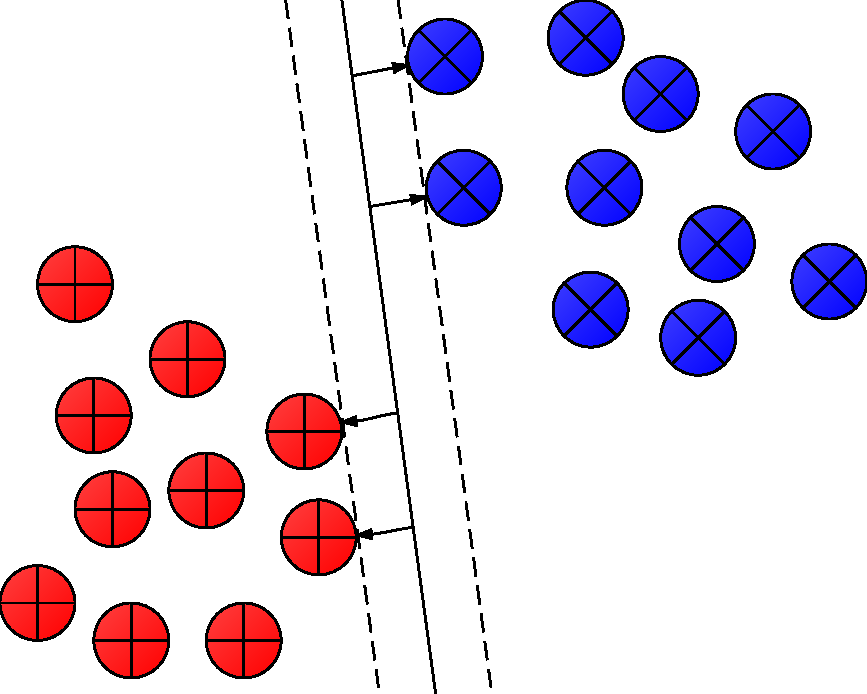
\includegraphics[width=5.5cm]{figures/SVM_small_margin.pdf}
    \label{fig:SVM_small_margin}
  }}
  \qquad
  \fbox{\subfloat[][\gls{svm} separated with a maximum margin between support vectors.]{
    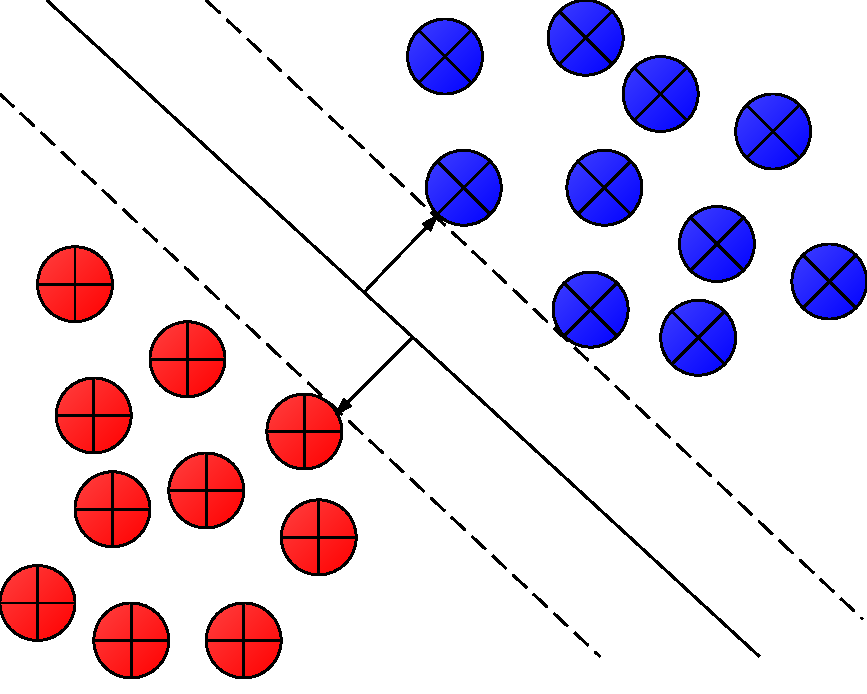
\includegraphics[width=5.5cm]{figures/SVM_maximum_margin.pdf}
    \label{fig:SVM_maximum_margin}
  }}
  \caption{Difference between small and maximum margins between support vectors.}
  \vspace{1mm}
  \footnotesize{\emph{As we can see in the two above examples, there are two categories in the feature space with a solid line separating them, this is called the ``hyperplane''. The dotted lines represent the distance to the closest vector from the hyperplane, the distance between both dotted lines is also called the ``margin''. ``Support vectors'' are the vectors that are touching the margin. The goal of a \gls{svm} is to maximizing the distance between support vectors of opposite categories using the hyperplane. There is a clear difference in the distance separating support vectors in the above examples, with the maximum margin~\subref{fig:SVM_maximum_margin} being a better solution then the small margin~\subref{fig:SVM_small_margin}.}}
  \vspace{2mm}
  \hrule
  \label{fig:SVM_margin}
\end{figure}

A \gls{svm} is an example of a linear discrimination machine learning technique and assumes that \emph{``\ldots instances of a class are linearly separable from instances of other classes''}~\cite{ALP04}. Traditionally, \gls{svm}s have been used for two-group classification problems~\cite{CV95} but have also been generalized to \emph{n}-group classification problems. The dataset used in \gls{svm} is applied to a \emph{feature space} that consists of a set of \emph{vectors} (a row of data in the dataset), with each vector containing a set of \emph{attributes} (the values that define the vector). In Figure~\ref{fig:SVM_margin} we have a \gls{svm} example with each vector having two predictor variables (\emph{x} and \emph{y} coordinates). A \gls{svm} attempts to find the maximum margin space between support vectors of opposite categories, which results in the optimal hyperplane. The optimal hyperplane is chosen over other as \emph{``Intuitively, we would expect this boundary to generalize well as opposed to the other possible boundaries.''}~\cite{Gun98}.

\begin{figure}[t!]
  \centering
  \fbox{\subfloat[][A \gls{svm} that has a non-linear separation between two categories.]{
    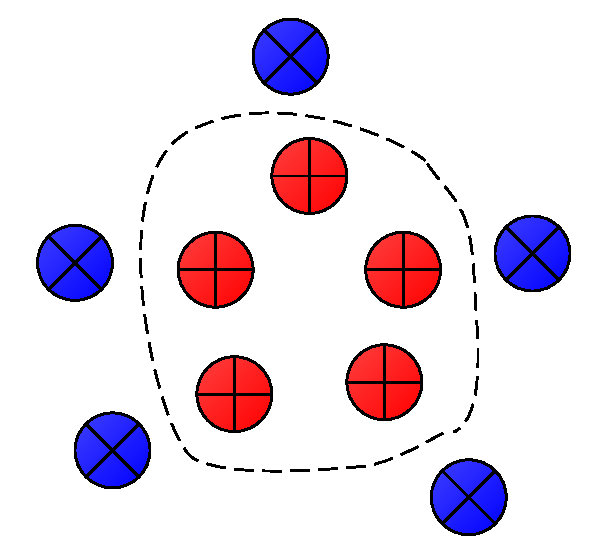
\includegraphics[width=5.5cm]{figures/SVM_non-linear.pdf}
    \label{fig:SVM_non-linear}
  }}
  $\xrightarrow{\texttt{Kernel Function}}$
  \fbox{\subfloat[][A \gls{svm} that is now linearly separable due to using a kernel function.]{
    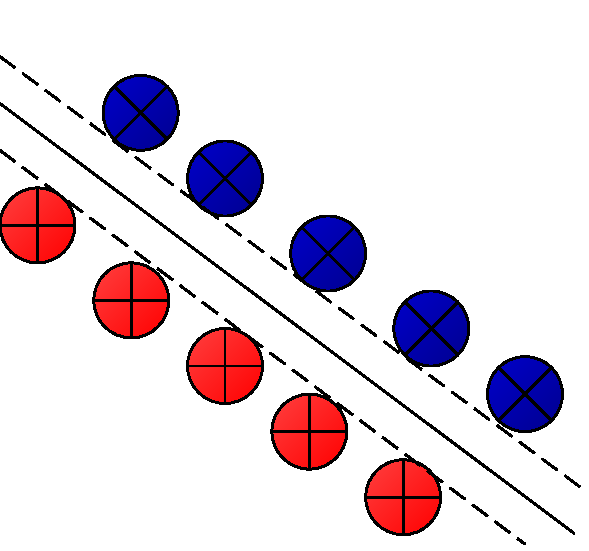
\includegraphics[width=5.5cm]{figures/SVM_kernel_function.pdf}
    \label{fig:SVM_kernel_function}
  }}
  \caption{Linearly separating non-linear using a kernel function.}
  \vspace{1mm}
  \footnotesize{\emph{As we can see in Figure~\ref{fig:SVM_non-linear_kernel} two example of \gls{svm}s are illustrated. A non-linear hyperplane is required in~\subref{fig:SVM_non-linear} to properly separate the two categories. \gls{svm}s attempt to linearly separate the feature space, in this case it is possible to map the vectors to a higher dimension using a \emph{kernel function}. In the above example a kernel function is used to map~\subref{fig:SVM_non-linear} to~\subref{fig:SVM_kernel_function} which results in a higher dimension such that each vector now has a radius value (distance from the center to the edge). As we can see in~\subref{fig:SVM_kernel_function} it is now linearly separable when the feature space is mapped to a higher dimension (from two-dimensions to three-dimensions).}}
  \vspace{2mm}
  \hrule
  \label{fig:SVM_non-linear_kernel}
\end{figure}

In some cases a linear separation is not possible in the feature space, for example in Figure~\ref{fig:SVM_non-linear_kernel}. It is possible to map the vectors to a higher dimension such that the feature space now becomes linearly separable. The separating hyperplane is always of \emph{n}-1 dimensions (e.g., two dimensional data is separated with a one dimensional line). Several kernel functions exist, though the \gls{rbf} kernel is highly recommended by the authors of LIBSVM~\cite{HCL03}. Kernels have parameters that govern how they form their corresponding hyperplane. The \gls{rbf} kernel has a \emph{gamma} parameter that governs the flexibility of the hyperplane. If the hyperplane is too flexible (i.e., follows the contour of the data too strictly) then it runs the risk of being overfitted for the given data~\cite{BW10}. Overfitting can lower the ability of a classifier to generalize. \gls{svm} handle this first with the maximum margin distance which allows some flexibility in adding new vectors to the feature space. Secondly, the concept of \emph{cost} is also present in \gls{svm}. If there is a low cost then the the \gls{svm} will allow some mis-classifications (within a distance from the hyperplane using a function of cost)~\cite{BW10}. A higher cost value will reduce the number of mis-classifications, but may create a model that does not generalize outside of the training data.

Considering the following criteria for \gls{svm}s we can distinguish between several different implementations from a user perspective:

\begin{itemize}
  \item \textbf{Inception Year}: the year the tool was released to the public.
  \item \textbf{Multiple-Group}: whether the tool supports multiple group classification problems, in addition to binary group classification.
  \item \textbf{Cross-Validation}: whether the tool supports cross-validation.
  \item \textbf{Measures}: whether the tools supports performance measures to aid in evaluation of classification accuracy.
  \item \textbf{Command-Line}: whether a tool has support to be ran via a command-line interface.
  \item \textbf{Open Source}: whether a tool's source code is open source and freely available to modify.
  \item \textbf{Academic Tool}: whether a tool was developed from an academic research group, otherwise industry or community developed.
\end{itemize}

\begin{table}[t!]
    \centering
    \rowcolors{1}{gray!30}{gray!20}
    \begin{threeparttable}
      \begin{tabular}{|l|l|l|l|}
        \rowcolor[RGB]{169,196,223}
        \hline & \textbf{SVM$^{light}$~\cite{Joa99}} & \textbf{LS-SVMlab~\cite{SV99, PSV+02}} & \textbf{LIBSVM~\cite{CL11}}  \\
        \hline \cellcolor[RGB]{169,196,223} \textbf{Inception Year} & 1999 & 1999 & 2000  \\
        \hline \cellcolor[RGB]{169,196,223} \textbf{Multiple-Group} & No\tnote{a} & Yes & Yes \\
        \hline \cellcolor[RGB]{169,196,223} \textbf{Cross-Validation} & Yes\tnote{e} & Yes & Yes \\
        \hline \cellcolor[RGB]{169,196,223} \textbf{Measures} & No\tnote{b} & Yes & No\tnote{c} \\
        \hline \cellcolor[RGB]{169,196,223} \textbf{Command-Line} & Yes & No\tnote{d} & Yes\tnote{f} \\
        \hline \cellcolor[RGB]{169,196,223} \textbf{Open Source} & Yes & Yes & Yes \\
        \hline \cellcolor[RGB]{169,196,223} \textbf{Academic Tool} & Yes & Yes & Yes \\
        \hline
      \end{tabular}
      \begin{tablenotes}
        \item[a] There is an alternative tool of the same family that allows this (SVM$^{multiclass}$).
        \item[b] There is an alternative tool of the same family that allows this only on binary classification (SVM$^{perf}$).
        \item[c] There is an external extension which allows this only for binary classification.
        \item[d] Is a MATLAB toolkit, though it is possible to run a MATLAB script via a \gls{cli}.
        \item[e] Performs a \emph{Leave-One-Out} cross-validation, which is a \emph{n}-fold cross-validating given a \emph{n} vectors in the feature set.
      \end{tablenotes}
    \end{threeparttable}
    \caption{Basic comparison of different \gls{svm} implementations from a user perspective.}
    \vspace{2mm}
    \hrule
    \label{tab:svm_tools}
  \end{table}

Using this criteria we provide a comparison of a different \gls{svm} implementations in Table~\ref{tab:svm_tools}. We can see various aspects of different \gls{svm} implementations, for example all three of these \gls{svm}s are open source academic tools that support cross-validation. SVM$^{light}$ does not support multiple-group classification, though it does have an alternative tool that does allow this. LS-SVMlab has the ability to gather perform measure, though it also works as a MATLAB toolkit.


\section{Software Metrics}
\label{sec:background_metrics}
Metrics are measurements of a system, which can provide insight in describing/understanding the system. Goodman defines software metrics as \emph{``The continuous application of measurement-based techniques to the software development process and its products to supply meaningful and timely management information, together with the use of those techniques to improve that process and its products''}~\cite{Goo93}. Measurements can be further defined using the following definitions~\cite{Fen94}:

\begin{itemize}
  \item \textbf{Entity:} Represents an object or event.
  \item \textbf{Attribute:} Represents a feature or property of an \emph{entity}.
  \item \textbf{Model:} Represents a specific viewpoint of an \emph{attribute}.
\end{itemize}

With respect to software metrics we can consider a multitude of entities such as the source code, the test cases, the bug reports and more. There are many possible attributes that can be used for any entity, it just has to be a repeatable and measurable property. A measurable attribute is not sufficient as there might be different views on how to interpret the attribute. For example, using a programs source code as the entity with the size in lines of code being the attribute, how do we view/represent size in this case? Should we include blank lines and/or comments, are we considering logical lines, physical lines? A model is used to specify the specific viewpoint of the attribute, with respect the the previous question we might view size with respect to physical lines that exclude blank lines and comments.

As mentioned there are a number of software metric entities available. With respect to source code as an entity there are a number of attributes that can represent structural characteristics of the source code as detailed in Section~\ref{subsec:background_source_code_metrics}. We also consider the test suite as an entity in Section~\ref{subsec:background_test_suite_metrics}, which is still ultimately code though also contains attributes specific to coverage. More software metrics entities are present (e.g., software development life-cycle, bug report(s), program execution~\cite{SS08}) that we do not explain in this chapter as it is not required as background material.


\subsection{Source Code Metrics}
\label{subsec:background_source_code_metrics}
In general, software metrics can be used to measure a number of qualities of a software system. In particular, source code metrics give insight into structural aspects of the system including it's complexity, size, as well as object-oriented attributes~\cite{McCa76, Kan02, HWY09, Hend95, SRD12}. Chidamber et al. presented a suite of object-oriented metrics~\cite{CK94}, around the same time Abreu et al. also presented the MOOD object-oriented suite~\cite{AC94}. Source code metrics are typically extracted from the source code using static analysis techniques. Some metrics like \emph{defect density} make use of external bug reports along with the source code to indicate problematic modules~\cite{FP98}. 

For the scope of this thesis we are only considering the Java programming language, which has object-oriented features. This means that source code metrics can be acquired at different scope-levels (i.e., method, class, package, project). For example, we can calculated the cyclomatic complexity~\cite{McCa76} of a method by simply counting the number of decisions points (i.e., different decisions of control statements). We can also calculate the nested block depth of a method, which is determined by the number of nested blocks (i.e., control statements). From a class-level perspective we can measure the number of methods and attributes the class contains. We can also measure the depth of the class in respect to its inheritance tree. At a higher level we start to consider the number of classes within a package, along with measuring coupling inside and outside of the package. These metrics can be used to alert developers if a specific class/method could be problematic. If these metrics reach extreme points (i.e., complex method, large class, high coupling) they can become \emph{code smells} (i.e., source code that is hard to read and maintain) that should be refactored~\cite{FB99}.


\subsection{Test Suite Metrics}
\label{subsec:background_test_suite_metrics}
The source code of a software system is one of the most important artifacts of the system. From a testing perspective the test suite is very important as it ensures the correctness of the \gls{sut}. Using the test suite as an entity for software metrics presents a number of attributes to be observed. For instances, the size of the test suite in terms of individual test cases or the the complexity of the test cases themselves. As test cases at a unit testing level are just source code anyways it is possible to borrow similar attributes from the source code metrics entity (see Section~\ref{subsec:background_source_code_metrics}). As mentioned in Section~\ref{sec:introduction_motivation}, coverage can also assess what parts of the source code are exercise by the test suite~\cite{ZHM97}. Coverage metrics is one of the more common test suite metrics, as it measures the relationship between the test suite and source code.


\section{Summary}
\label{sec:background_summary}
In this chapter we have covered the following background topics for the research presented in this thesis:

\begin{itemize}
  \item In Section~\ref{sec:background_mutation_testing} we covered what is mutation testing and how it relates to test suite effectiveness with respect to fault detection adequacy. We explored various sets of mutation operators with examples for method- and class-level mutation. A set of Java specific mutation tools was also discussed  for comparison.
  \item In Section~\ref{sec:background_machine_learning} we covered what machine learning and the differences between supervised and unsupervised classification. We specifically covered common performance measures and how \gls{svm}s work.
  \item In Section~\ref{sec:background_metrics} we covered software metrics -- specifically source code and test suite metrics. We explain how source code metrics can be used to identify \emph{code smells} and some examples of these metrics. We also explain several approaches to test suite metrics using a combination of source code metrics on JUnit test cases as well as coverage metrics.
\end{itemize}
